%%%%%%%%%%%%%%%%%%%%%%%%%%%%%%%%%%%%%%%%%%%%%%%%%%%%%%%%%%%%%%%%%%%%%%%%%%%
%%%                                                                     %%%
%%%   LaTeX template voor het verslag van P&O: Computerwetenschappen.   %%%
%%%                                                                     %%%
%%%   Opties:                                                           %%%
%%%     tt1     Tussentijdsverslag 1                                    %%%
%%%     tt2     Tussentijdsverslag 2                                    %%%
%%%     tt3     Tussentijdsverslag 3                                    %%%
%%%     eind    Eindverslag                                             %%%
%%%                                                                     %%%
%%%   2 oktober 2012                                                    %%%
%%%   Versie 1.0                                                        %%%
%%%                                                                     %%%
%%%%%%%%%%%%%%%%%%%%%%%%%%%%%%%%%%%%%%%%%%%%%%%%%%%%%%%%%%%%%%%%%%%%%%%%%%%

\documentclass[tt3]{penoverslag}

%%% PACKAGES
\usepackage{lipsum}
\usepackage{gensymb}
\usepackage [dutch] {babel}
\usepackage{graphicx}
\usepackage{amsmath}
\usepackage{listings}
\usepackage{subcaption}

\begin{document}

% == VOORPAGINA == %
\team{Zilver} % teamkleur
\members{Sam Gielis\\
         Sophie Marien\\
         Toon Nolten\\
         Nele Rober\\
         Gerlinde Van Roey\\
         Maxim Van Mechelen} % teamleden

\maketitlepage

% == ABSTRACT EN INHOUDSTAFEL == %
\begin{abstract}
\label{ssec:abstr} % 3 ok
Het P\&O-project bestaat eruit een robot autonoom een doolhof te laten verkennen. Dit verslag beschrijft de invulling die team Zilver aan het project gaf. De robot is voorzien van een lichtsensor en een ultrasone sensor. Deze staan vast gemonteerd en kunnen niet onafhankelijk van de robot bewegen. De aansturing van de robot gebeurt via bluetoothverbinding. Een Grafische User Interface (GUI) maakt deze aansturing op een gebruiksvriendelijke manier mogelijk. De GUI geeft de baan van de robot  weer. Ook een historiek van de sensorwaarden wordt weergegeven in de GUI.

De robot kan zich autonoom door een doolhof voortbewegen zonder op muren te botsen. Tijdens het rijden slaat de robot een map op van de doolhof. Op elke nieuwe tegel kijkt de robot rond en geeft de gedetecteerde muren door. Wanneer de hele doolhof verkend is, gebruikt de robot het \textit{A*}-algoritme om de kortste weg naar de finish te bepalen. De finish wordt aangegeven met een bepaalde barcode. Andere barcodes laten de robot een opdracht uitvoeren.

Om de afwijking op de aansturing te minimaliseren, ori\"enteert de robot zich regelmatig op een witte lijn. Zo blijft de robot steeds zo dicht mogelijk bij het midden van de tegels.

Een computerprogramma simuleert de werking van de robot. Het is voor de simulator mogelijk door een virtuele doolhof te rijden en deze op gelijkaardige wijze te verkennen. De sensorwaarden worden gesimuleerd, met een afwijking om de werkelijke robot zo goed mogelijk te benaderen, maar verder worden dezelfde algoritmes gebruikt. Dit laat toe de algoritmes te testen zonder de robot hiervoor te gebruiken.

\end{abstract}

\tableofcontents

%%figuur robot
%\begin{figure}[!hb]
%\begin{flushright}
%    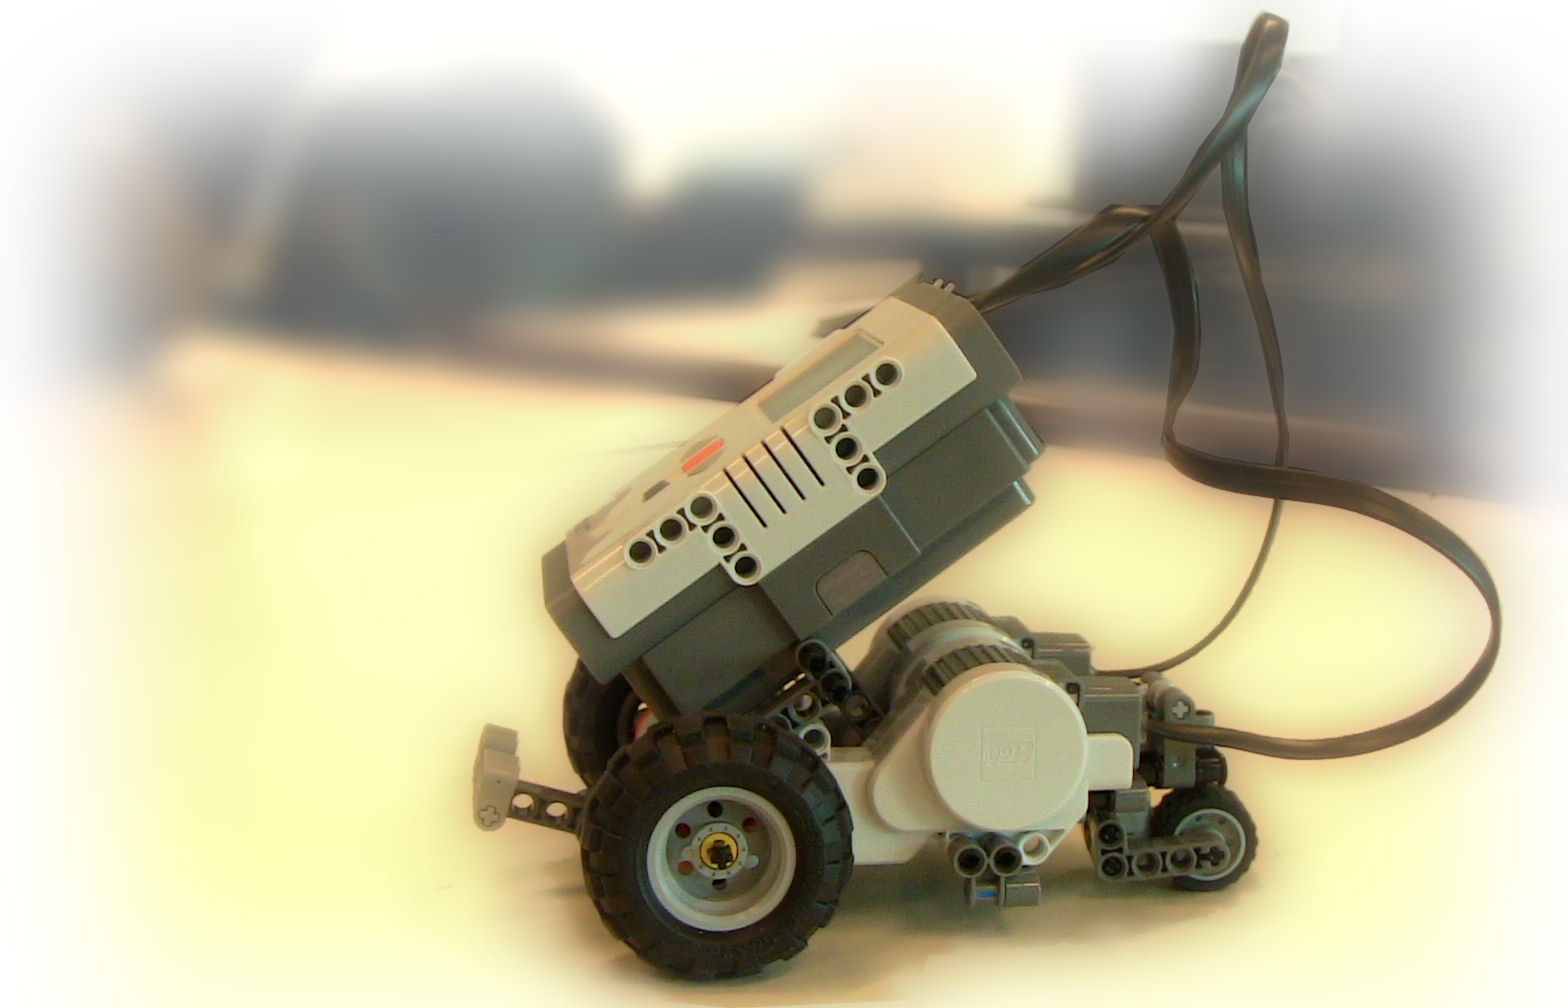
\includegraphics[width=1\textwidth]{robotFP}
%    \label{fig:robotFP}
%\end{flushright}
%\end{figure}


\newpage 

% == INLEIDING == %
\section{Inleiding} % 3 ok!
\label{ssec:inl}
In het kader van het vak 'Probleemoplossen en Ontwerpen: computerwetenschappen' wordt gewerkt rond autonome intelligente robots. Verschillende teams bouwen en programmeren een robot met behulp van LEGO Mindstorms. Deze robot moet uiteindelijk volledig autonoom een doolhof kunnen verkennen.\\
Op de derde demonstratie kan de robot alle taken van de vorige demonstratie nog steeds uitvoeren. De robot kan zich volledig autonoom voortbewegen. Wanneer de robot zich in een doolhof voortbeweegt, kan hij deze in kaart brengen. Bij het inlezen van barcodes voert de robot een bepaalde opdracht uit. Op het moment dat de volledige doolhof is ingelezen, bepaalt de robot de kortste weg naar zijn beginpositie en rijdt hier in hoge snelheid naartoe.

% == BOUW == %
\section{Bouw van de robot} % 3 ok
\label{sec:bouw}
LEGO Mindstorms \cite{mindstorms} biedt een bouwpakket voor een robot aan. Een NXT-microcomputer laat toe de robot te programmeren, met behulp van leJOS kan dit in Java.

% == fysieke bouw == %
\subsection{Fysieke bouw} % 3 ok
\label{ssec:fysbouw}
Bij het bouwen van de robot (zie figuur \ref{robot}) werd het ontwerpboekje gevolgd. Deze compacte samenstelling leek geen directe nadelen te hebben. Twee grote wielen worden elk met hun eigen motor aangestuurd. Een klein wiel achteraan zorgt ervoor dat de robot vlot kan draaien en wordt niet aangedreven. De sensoren (zie figuur \ref{fig:sensors}) werden als volgt ge\"installeerd: 

\begin{itemize}
\item \textit{lichtsensor:} vooraan en dicht tegen de grond.
\item \textit{ultrasone sensor:} bovenaan, naar voren kijkend. De sensor staat vast gemonteerd.
\item \textit{druksensoren:} aan beide zijkanten, \'e\'en aan de linkerkant en \'e\'en aan de rechterkant.
\end{itemize}

%figuur robot
\begin{figure}[tbp]
\begin{center}
    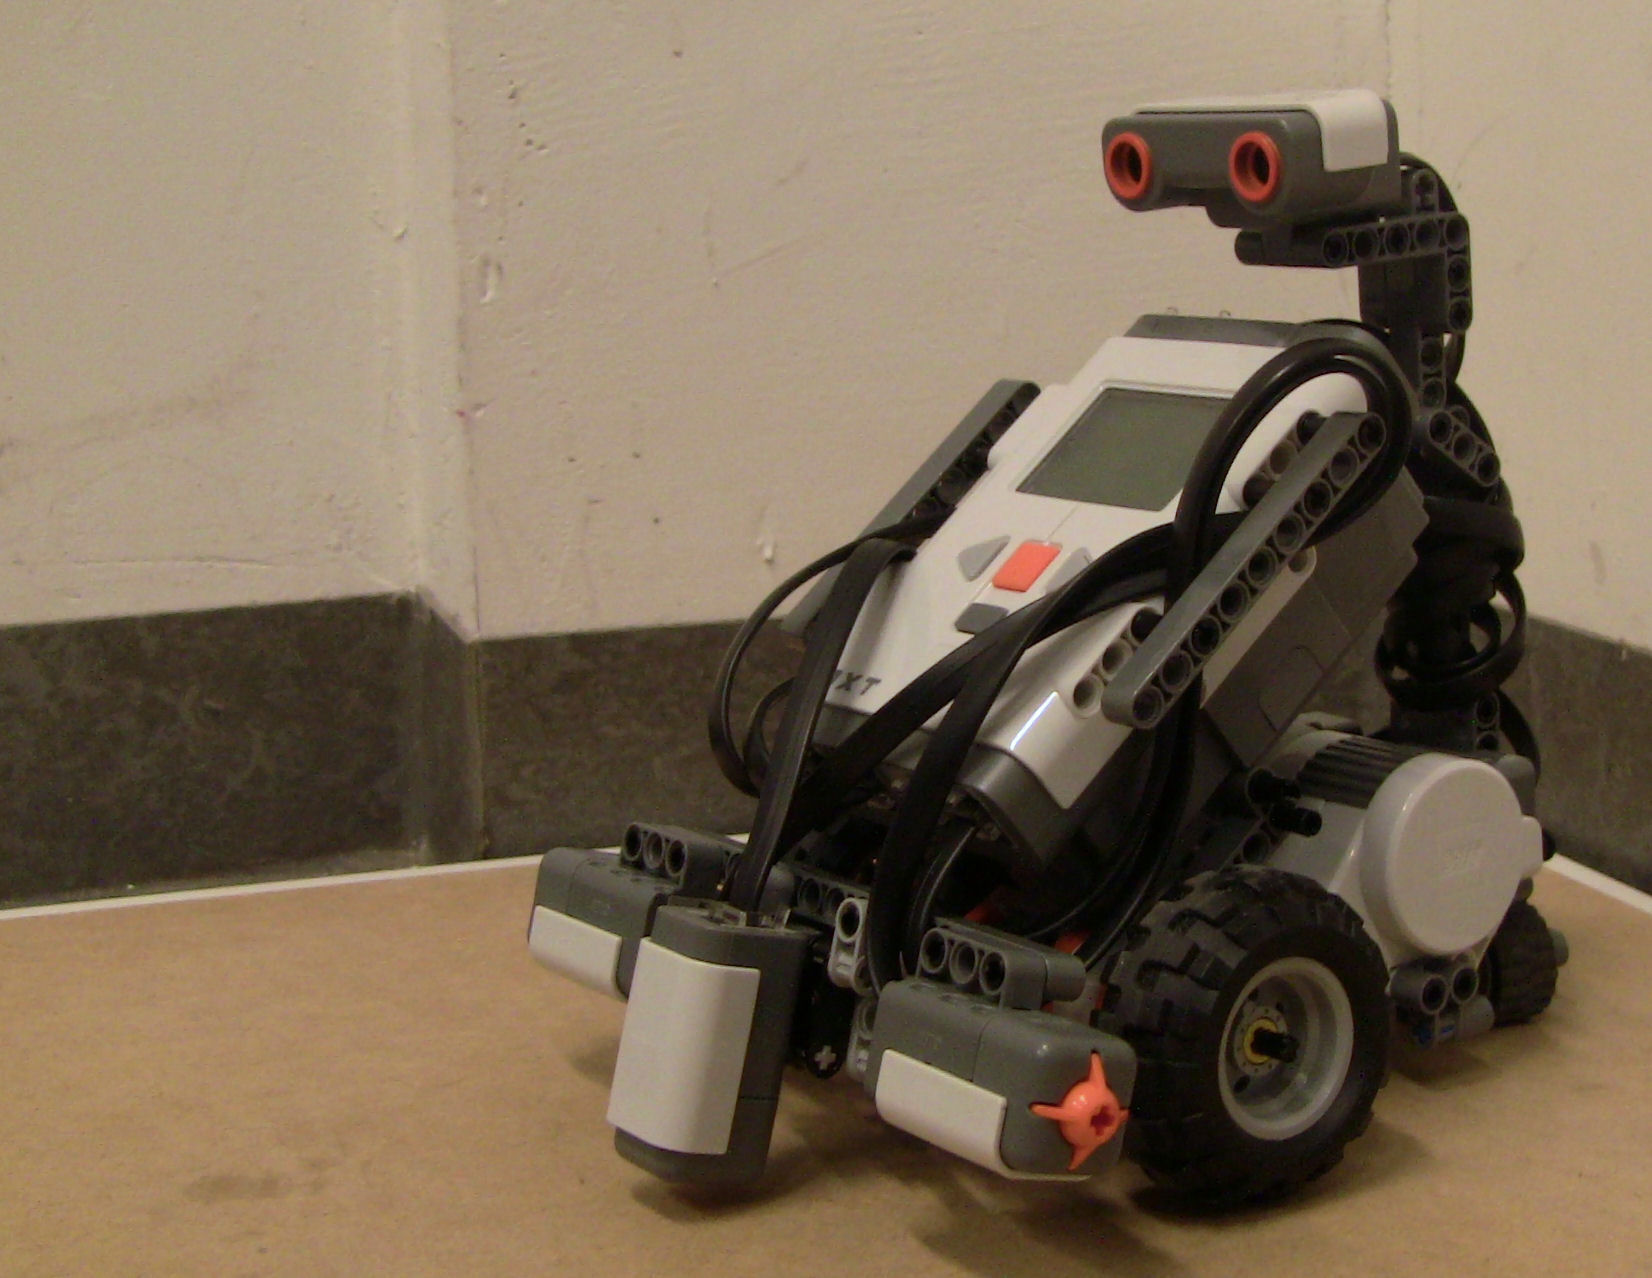
\includegraphics[width=0.8\textwidth]{robot}
    \caption{Robot}
    \label{robot}
\end{center}
\end{figure}


% figuur sensoren
\begin{figure}
        \centering
        \begin{subfigure}[h]{0.54\textwidth}
                \centering
                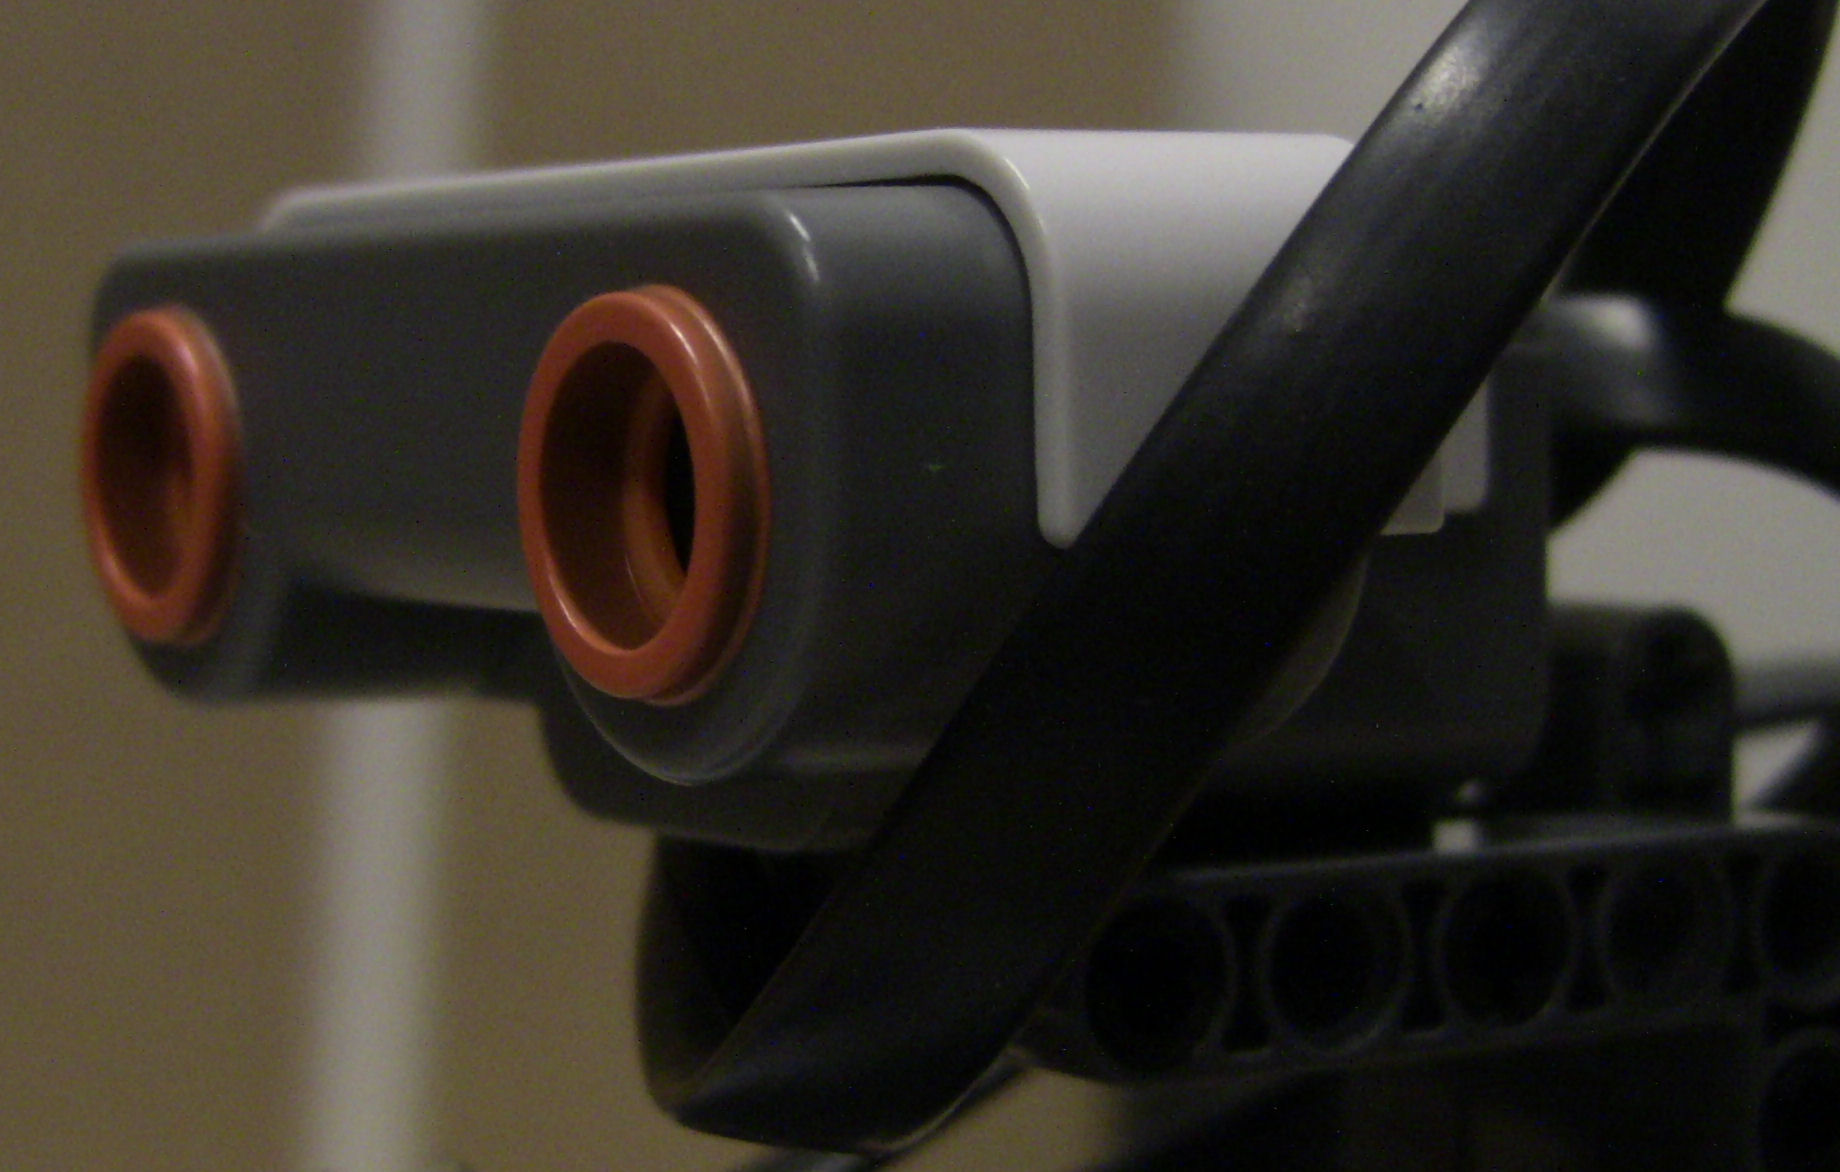
\includegraphics[width=\textwidth]{robotUS}
                \caption{Ultrasone sensor}
        \end{subfigure}%
        \begin{subfigure}[h]{0.46\textwidth}
                \centering
                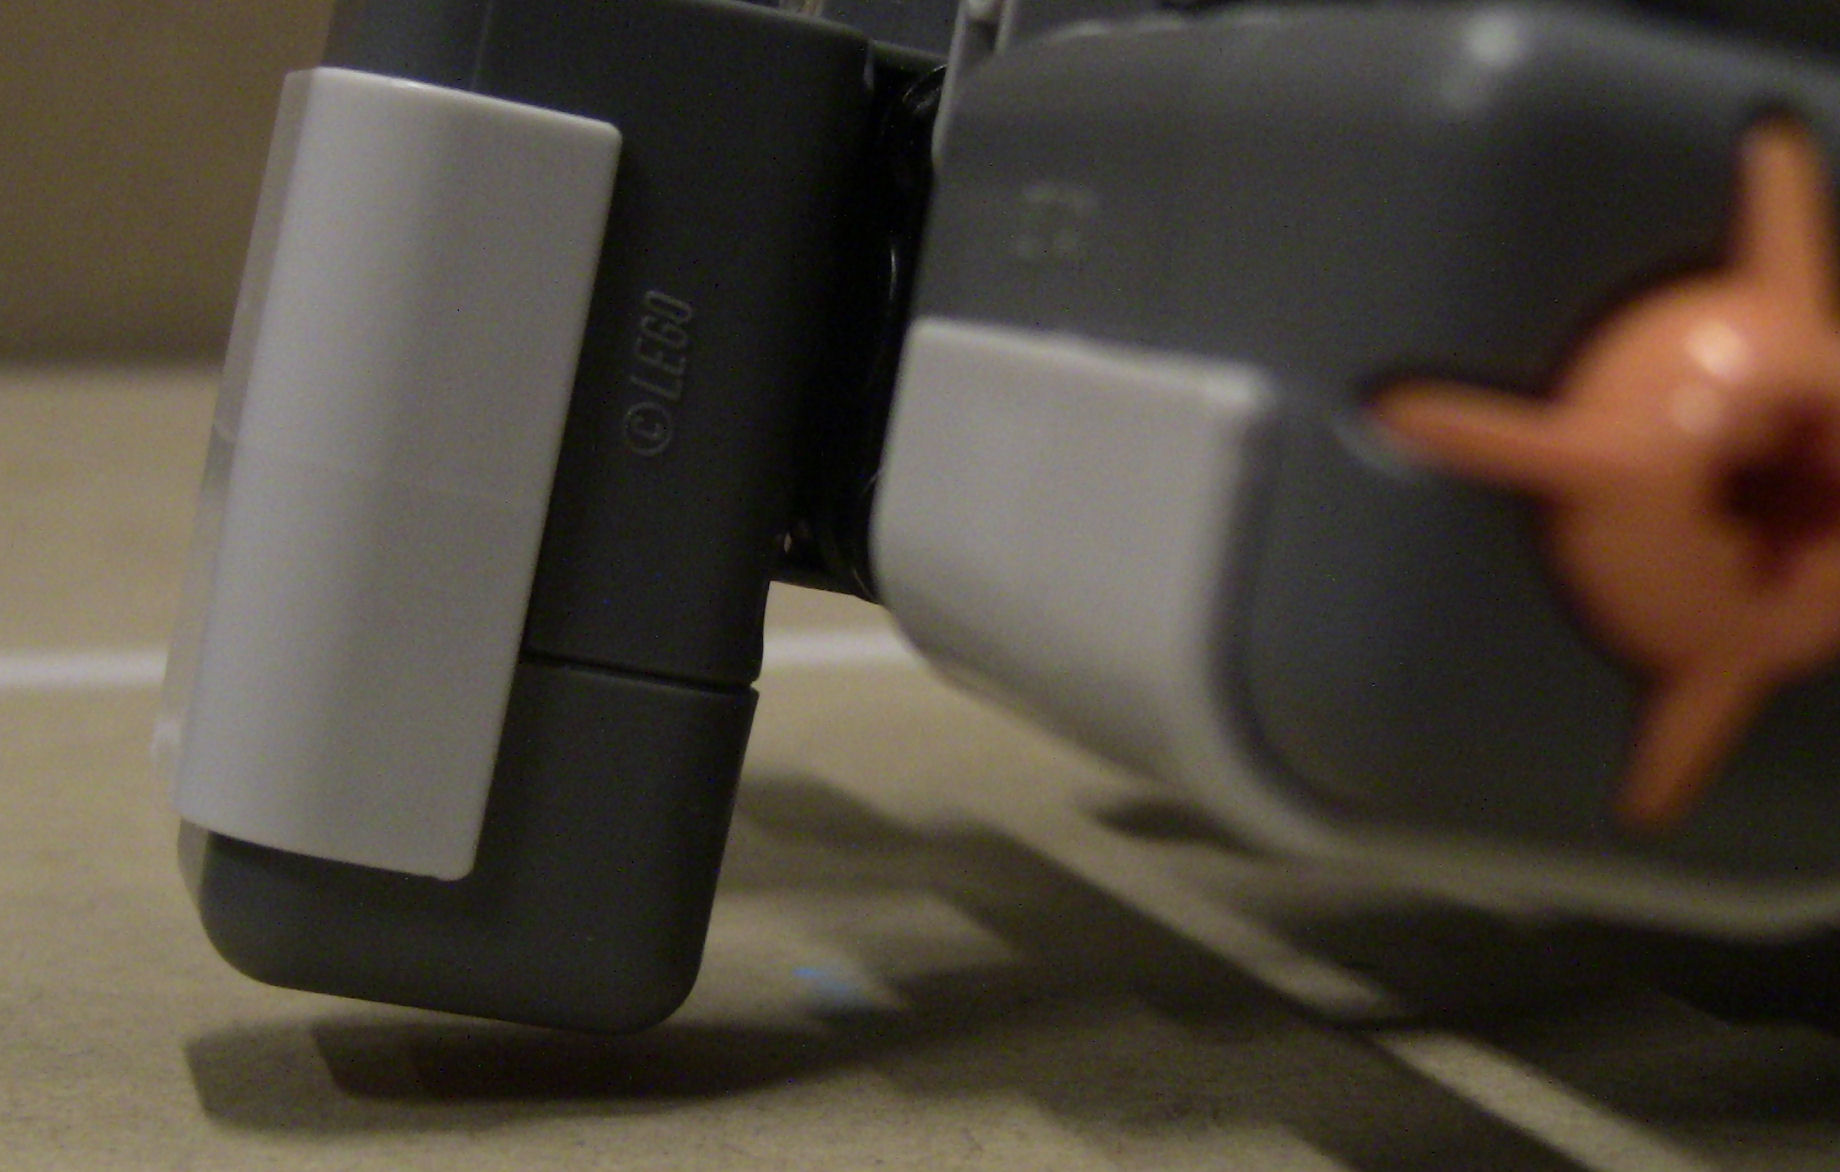
\includegraphics[width=\textwidth]{robotLSTS}
                \caption{Licht- en Druksensor}
        \end{subfigure}
        \label{fig:sensors}
        \caption{Sensoren}
\end{figure}


Een alternatieve opstelling bestaat erin de ultrasone sensor op een derde motor te monteren zodat deze onafhankelijk van de robot kan ronddraaien. Opdat hier plaats genoeg voor is, moet de NXT plat gelegd worden met de wielen aan weerszijden. Dit vraagt echter een nieuwe calibratie. Bovendien zou de meetwaarde van de ultrasone sensor afhangen van zijn positie ten opzichte van de robot, wat het interpreteren moeilijker maakt. Voor deze opstelling werd daarom niet gekozen.


% == calibratie == %
\subsection{Calibratie van de motoren} % 3 MEETWAARDEN + BOXPLOT
\label{ssec:calibM}
De robot wordt aangedreven door twee motoren, elk verbonden met \'e\'en van de twee grote wielen. De aansturing gebeurt door te bepalen hoeveel graden de wielen moeten draaien. Beide motoren kunnen onafhankelijk ingesteld worden. De robot kan vooruit bewegen en rond zijn as. De resultaten van de calibratie worden weergegeven in tabel \ref{tab:resultCalibM}.

%resultaten meetwaarden
\begin{table}[hb]
\begin{center}
    \begin{tabular}{  l || c | c | c }
     & linkerwiel & rechterwiel & aantal graden \\ \hline \hline
    1 cm vooruit & voor & voor & 20,8\degree
    \\ \hline
    1 cm achteruit & achter & achter & 20,8\degree
    \\ \hline
    180\degree draaien linksom & achter & linker & 701\degree \\ \hline
    180\degree draaien rechtsom & voor & achter & 701\degree \\
    \end{tabular}
    \caption{Resultaten calibratie motoren}
    \label{tab:resultCalibM}
\end{center}
\end{table}



\subsubsection{E\'en cm vooruit bewegen: bepalen van $x$} % 3 te weinig meetwaarden
\label{ssec:calibMx}
De parameter $x$ bepaalt het aantal graden dat de wielen moeten draaien opdat de robot \'e\'en cm vooruit beweegt.\\
Een schatting voor $x$ via de $diameter$ (in centimeter) gebeurt als volgt:

\begin{equation*}
x_{0} \approx \frac{360}{\pi \cdot diameter}
\end{equation*}

Een verdere nauwkeurigere bepaling van $x$ gebeurt via tests.\\
De robot wordt naast een lintmeter geplaatst en krijgt opdracht beide wielen $100 \cdot x$ graden te laten draaien. Bij een perfect gekozen waarde voor $x$, legt de robot precies \'e\'en meter af. Indien niet, wordt $x$ aangepast en wordt de test herhaald tot een voldoende nauwkeurig resultaat bekomen wordt.
% ONTBREEKT: x0 + afwijking op 1m; x1 + afwijking; x2 + afwijking + ...

Een volgende test bestaat eruit de robot beide wielen tien maal $10 \cdot x$ graden te laten draaien. Een boxplot van de totaal afgelegde afstand wordt weergegeven in figuur \ref{fig:calibM}. Wanneer geen afwijking op \'e\'en meter wordt waargenomen, heeft het starten en stoppen geen invloed op de totale afgelegde afstand. Dit blijkt echter wel het geval. In verdere algoritmes wordt hier rekening mee gehouden. De robot legt steeds \'e\'en lange afstand af in plaats van vele korte.\\
Uit deze test blijkt bovendien dat de robot een afwijking naar links heeft wanneer hij rechtdoor rijdt. De boxplot van deze afwijking wordt eveneens weergegeven in figuur \ref{fig:calibM}.
% ONTBREEKT: MEETWAARDEN VAN 1x100CM ter vergelijking


\subsubsection{Volledig rond de as draaien: bepalen van y} % 3 te weinig meetwaarden
\label{ssec:calibMy}
De parameter $y$ bepaalt het aantal graden dat de wielen moeten draaien opdat de robot 360\degree rond zijn as zou draaien. Beide wielen draaien hierbij in tegengestelde richting.\\
Een schatting voor $y$ via de diameter van het wiel, met $as_{robot}$ (afstand tussen beide wielen) en $diameter$ in centimeter:

\begin{equation*}
y_{0} \approx \frac{(2 \cdot \pi) \cdot (as_{robot}/2)}{diameter_{wiel}/2}
\end{equation*}

De robot wordt naast een lijn geplaatst en krijgt de opdracht zijn wielen $y$ graden in tegengestelde richtingen te laten draaien. $y$ wordt aangepast tot de robot na het draaien opnieuw precies naast de lijn uitkomt.
% ONTBREEKT: y0 + afwijking op 360°; y1 + afwijking; y2 + afwijking + ...


Door de robot in stappen rond zijn as te laten draaien ($4x90\degree$) kan de invloed van het starten en stoppen van de motoren bepaald worden. Figuur \ref{fig:calibM} geeft een boxplot van de gemeten afwijkingen op 180\degree. De algoritmes houden met deze afwijking rekening. Nadat de robot naar \'e\'en kant gedraaid heeft, draait hij, zo mogelijk, evenveel graden naar de andere kant terug. Op deze manier wordt de afwijking ongedaan gemaakt.
% ONTBREEKT: MEETWAARDEN VAN 1x180° ter vergelijking


% boxplots calibratie motoren
\begin{figure}
        \centering
        \begin{subfigure}[h]{0.32\textwidth}
                \centering
                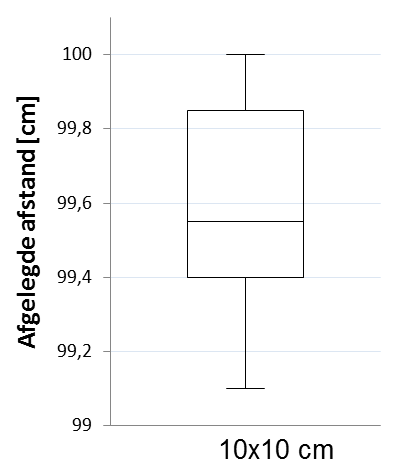
\includegraphics[width=\textwidth]{boxMrechtdoor10x10}
                \caption{Afgelegde afstand rechtdoor}
        \end{subfigure}%
        \begin{subfigure}[h]{0.32\textwidth}
                \centering
                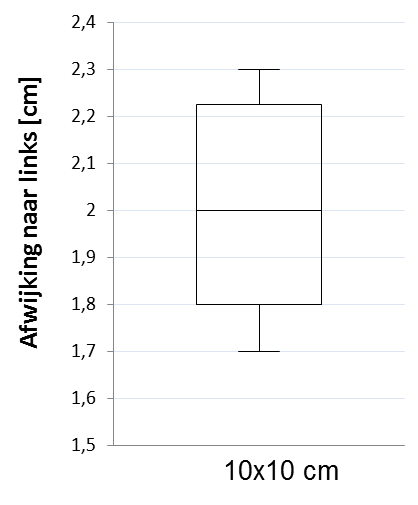
\includegraphics[width=\textwidth]{boxMlinks10x10}
                \caption{Afwijking naar links}
        \end{subfigure}%
        \begin{subfigure}[h]{0.32\textwidth}
                \centering
                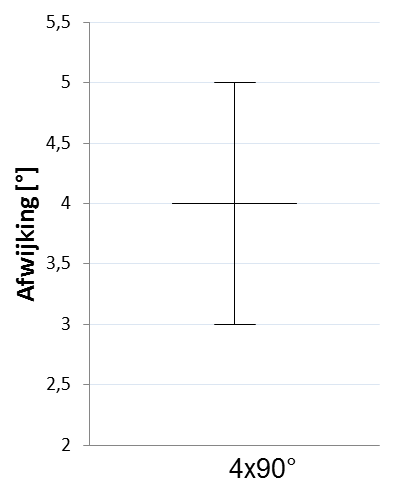
\includegraphics[width=\textwidth]{boxMgraden4x90}
                \caption{Afwijking op $360 \degree$}
        \end{subfigure}
 \caption{Boxplots calibratie motoren.}
\label{fig:calibM}
\end{figure}


\subsection{Calibratie van de lichtsensor} % 3 ok
\label{ssec:calibLS}
De lichtsensor meet de lichtintensiteit van de omgeving. De sensor kan zelf ook een rood licht uitsturen. Hoe minder licht gereflecteerd wordt door de omgeving, hoe donkerder de omgeving. Op deze manier kunnen de meetwaarden ge\"interpreteerd worden als witte of zwarte lijnen.\\
De lichtsensor wordt in verschillende omstandigheden getest: bij direct kunstlicht, in de schaduw, terwijl de robot rijdt en terwijl hij stilstaat. Dit voor alle soorten ondergrond die in de doolhof voorkomen: een paneel, een witte lijn en een zwarte lijn. Boxplots worden weergegeven in figuur \ref{fig:calibLS}. Deze toont dat het gemiddelde enkel bij een zwarte lijn afhangt van de omstandigheden. De afwijking wordt echter sterk bepaald door het feit of de robot rijdt of stilstaat. Bij het simuleren en het interpreteren van de meetwaarden wordt hier rekening mee gehouden.

% boxplots calibratie lichtsensoren
\begin{figure}
        \centering
        \begin{subfigure}[h]{0.32\textwidth}
                \centering
                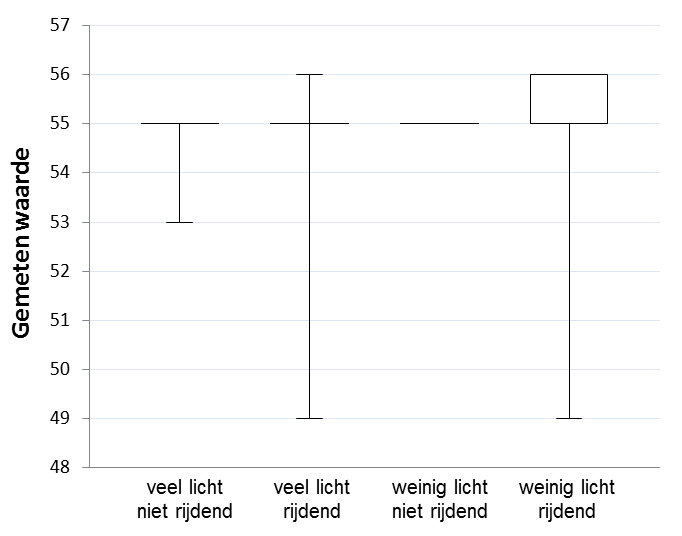
\includegraphics[width=\textwidth]{boxLSwit}
                \caption{Witte lijn}
        \end{subfigure}%
        \begin{subfigure}[h]{0.32\textwidth}
                \centering
                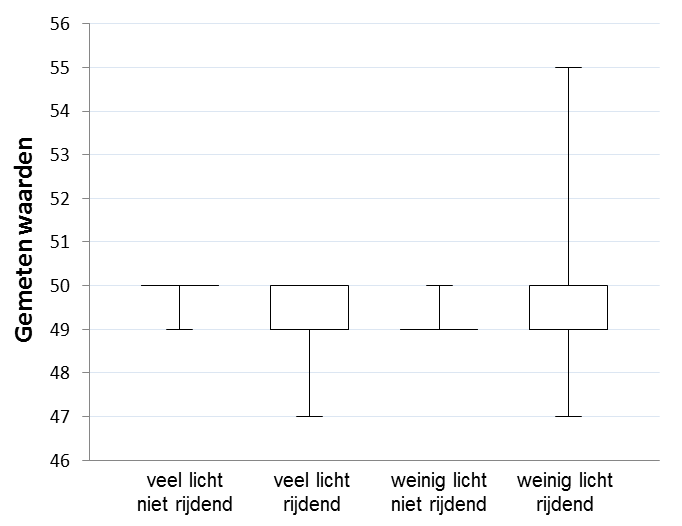
\includegraphics[width=\textwidth]{boxLSpaneel}
                \caption{Paneel}
        \end{subfigure}%
        \begin{subfigure}[h]{0.32\textwidth}
                \centering
                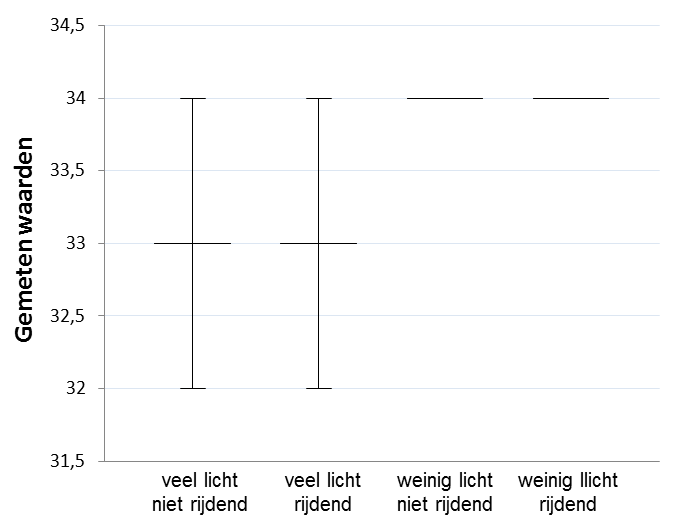
\includegraphics[width=\textwidth]{boxLSzwart}
                \caption{Zwarte lijn}
        \end{subfigure}
 \caption{Boxplots calibratie lichtsensor.}
\label{fig:calibLS}
\end{figure}

%%resultaten lichtsensor
%\begin{table}[hb]
%\begin{center}
%    \begin{tabular}{ c | r || c | c | c | c | c | c | c | c }
%     & & WVN & WVR & WWN & WWR & PVN & PVR & PWN & PWR \\ \hline \hline
%    $Q_{0}$ & min & 53 & 49 & 55 & 49 & 49 & 47 & 49 & 47 \\ \hline
%    $Q_{0.25}$ & 1/4 & 55 & 55 & 55 & 55 & 50 & 49 & 49 & 49 \\ \hline
%    $Q_{0.5}$ & med & 55 & 55 & 55 & 55 & 50 & 49 & 49 & 49 \\ \hline
%    $Q_{0.75}$ & 3/4 & 55 & 55 & 55 & 56 & 50 & 50 & 49 & 50\\ \hline
%    $Q_{1}$ & max & 55 & 56 & 55 & 56 & 50 & 50 & 50 & 55 \\ \hline \hline
%     & gem & 54.995 & 55.0261 & 55 & 55.0645 & 49.99688 & 490.2918 & 49.1 & 49.388\\ \hline
%     & st.dev. & 0.10025 & 0.96642 & 0 & 1.025 & 0.055815 & 0.58241 & 0.30015 & 0.95622 \\
%    \end{tabular}
%    \caption{Resultaten lichtsensor, witte ondergrond en paneel ondergrond}
%    \label{tab:resultCalibM}
%\end{center}
%\end{table}
%
%%resultaten lichtsensor
%\begin{table}[hb]
%\begin{center}
%    \begin{tabular}{ c | r ||  c | c | c | c }
%     & & ZVN & ZVR & ZWN & ZWR\\ \hline \hline
%    $Q_{0}$ & min & 32 & 32 & 34 & 34 \\ \hline
%    $Q_{0.25}$ & 1/4 & 33 & 33 & 34 & 34 \\ \hline
%    $Q_{0.5}$ & med & 33 & 33 & 34 & 34 \\ \hline
%    $Q_{0.75}$ & 3/4 & 33 & 33 & 34 & 34\\ \hline
%    $Q_{1}$ & max & 34 & 34 & 34 & 34 \\ \hline \hline
%     & gem & 33.05 & 33.05 & 34 & 34 \\ \hline
%     & st.dev. & 0.27279 & 0.27279 & 0 & 0 \\
%    \end{tabular}
%    \caption{Resultaten lichtsensor, zwarte ondergrond}
%    \label{tab:resultCalibM}
%\end{center}
%\end{table}


\subsection{Calibratie van de ultrasone sensor} % 3 ok
\label{ssec:calibUS}
Een ultrasone sensor zendt ultrasone geluidsgolven uit. De golven weerkaatsen op een object dat zich binnen het bereik bevindt. Bij ontvangst van zijn eigen geluidsgolven, weet de robot dat er een object in de buurt is en door de tijd tuss uitzenden en ontvangen op welke afstand het object zich bevindt.\\

In het kader van een doolhof, kan een robot muren tegenkomen. Ook de paaltjes, die de muren omhoog houden, worden als object gedetecteerd. Om te vermijden dat de paaltjes als muur worden ge\"interpreteerd worden enkel meetwaarden kleiner dan 29 cm als muur beschouwd.

De afwijking van de ultrasone sensor wordt gemeten door de robot op een bepaalde afstand van een muur te zetten. Verschillende afstanden worden zo gemeten. Boxplots in figuur \ref{fig:calibUS} geven de gemeten waarden (boven de lijnen) ten opzichte van de werkelijke waarden weer. Hoewel de variantie op de gemeten waarde niet groot is, komt de gemiddelde gemeten waarde niet altijd overeen met de werkelijke afstand. Vooral voor afstanden kleiner dan 20 cm en groter dan 145 cm, wijkt de gemeten waarde af van de werkelijke waarde. Waarden buiten het interval [20,145] worden daarom niet als betrouwbaar veronderstelt.

% boxplots calibratie ultrasone sensor
\begin{figure}
        \centering
        \begin{subfigure}[h]{0.69\textwidth}
                \centering
                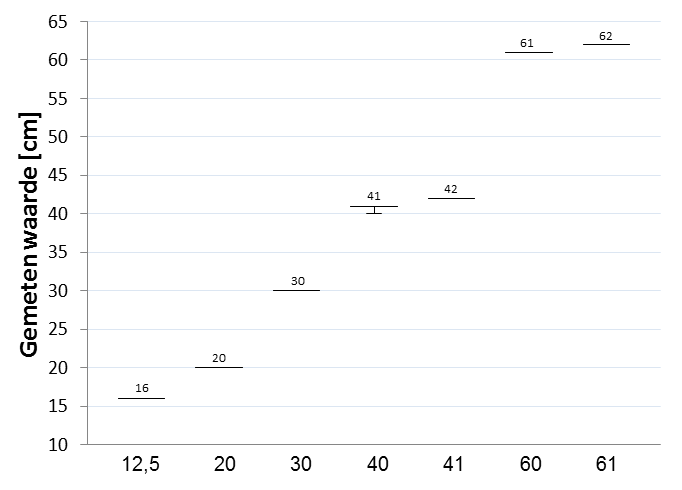
\includegraphics[width=\textwidth]{boxUS}
                \caption{meetwaarden}
        \end{subfigure}%
        \begin{subfigure}[h]{0.31\textwidth}
                \centering
                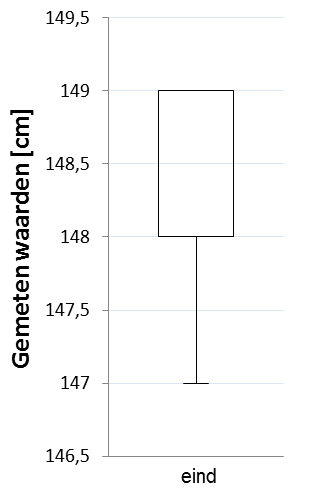
\includegraphics[width=\textwidth]{boxUSeind}
                \caption{laatste geldige meetwaarde}
        \end{subfigure}
 \caption{Boxplots calibratie ultrasone sensor.}
\label{fig:calibUS}
\end{figure}

%%resultaten lichtsensor
%\begin{table}[hb]
%\begin{center}
%    \begin{tabular}{ c | r || c | c | c | c | c | c | c | c | c | c | c | c }
%     & & 12.5 & 20 & 30 & 40 & 41 & 60 & 61 & eind\\ \hline \hline
%    $Q_{0}$ & min & 16 & 20 & 30 & 40 & 42 & 61 & 62 & 147 \\ \hline
%    $Q_{0.25}$ & 1/4 & 16 & 20 & 30 & 40 & 42 & 61 & 62 & 148 \\ \hline
%    $Q_{0.5}$ & med & 16 & 20 & 30 & 40 & 42 & 61 & 62 & 149 \\ \hline
%    $Q_{0.75}$ & 3/4 & 16 & 20 & 30 & 40 & 42 & 61 & 62 & 149\\ \hline
%    $Q_{1}$ & max & 16 & 20 & 30 & 40 & 42 & 61 & 62 & 149 \\ \hline \hline
%     & gem & 16 & 20 & 30 & 40.99571 & 42 & 61 & 62 & 148.5 \\ \hline
%     & st.dev. & 0 & 0 & 0 & 0.065512 & 0 & 0 & 0 & 0.565091 \\
%    \end{tabular}
%    \caption{Resultaten ultrasone sensor}
%    \label{tab:resultCalibM}
%\end{center}
%\end{table}


% == ALGORITMES == %
\section{Algoritmes} % 3 ?
\label{sec:algo}
Verschillende algoritmes zorgen ervoor dat de robot alle opdrachten kan uitvoeren.

% == veelhoek == %
%\subsection{Het rijden van een veelhoek} % 3 ?
%\label{ssec:algoVeelH}
%De robot en de simulator kunnen beiden een veelhoek rijden. Het aantal hoeken en de lengte van %de zijden kunnen via de GUI ingesteld worden. De robot en de simulator rijden een afstand, %draaien een bepaald aantal graden rond hun as, rijden weer dezelfde afstand,... Tot de %volledige veelhoek gereden is. 
%
%\lstset{frame=single, language=Java, caption=Veelhoek algoritme (pseudocode),
%   	label=code:algoVeelH, numbers=left, numberstyle=\footnotesize,
%		basicstyle=\sffamily, numbersep=5pt}
%\begin{lstlisting}
%Angle = (360.0/amtOfAngles)*100
%Voor i van 0 tot amtOfAngles
%	Beweeg lengthInCM vooruit
%	Draai angle
%\end{lstlisting}


% == witte lijn == %
\subsection{Het rechtzetten op een witte lijn} % 3 ?
\label{ssec:algoWitteL}
Indien regelmatig gecorrigeerd wordt op de calibratieafwijkingen kan de impact ervan geminimaliseerd worden. Deze correctie gebeurt door de witte lijnen als referentie te nemen en hier loodrecht op te ori\"enteren.
Onderstaand algoritme kan gebruikt worden wanneer de robot vlakbij een witte lijn staat (wanneer hij volledig rond zijn as draait zou hij de witte lijn moeten detecteren):

\lstset{frame=single, caption=Witte Lijn algoritme (pseudocode),
		label=code:algoWitteL, numbers=left, numberstyle=\footnotesize,
		basicstyle=\sffamily, numbersep=5pt}
\begin{lstlisting}
AngleTurned = 0

Draai naar rechts tot witte lijn.
Draai naar links tot witte lijn EN verhoog AngleTurned.
Draai AngleTurned/2 naar rechts.
\end{lstlisting}

Bij demo 3 is er iets veranderd aan het algoritme. Tijdens het testen zagen we dat als er een zwarte lijn op een witte streep stond (scheiding van twee tegels die tegen elkaar worden gezet), dat de robot zich niet loodrecht kon zetten op de witte lijn. Om dit tegen te gaan is ervoor gezorgd dat als de robot een witte lijn detecteert, hij er eerst helemaal overgaat en dan pas draait om zich loodrecht op de witte lijnen te plaatsen. Het resultaat was dat de robot zich veel beter recht zette op de witte lijn bij het testen.\\

Alternatief is het mogelijk te corrigeren op de muren, maar dan moet de robot zicht bevinden op een tegel die muren aan beide kanten bevat.


% == onderzoeken van het doolhof == %
\subsection{Onderzoeken van het doolhof} % 3 ?
\label{ssec:algoOnderzDoolhof}
De robot kan een volledige doolhof autonoom verkennen. Elke tegel die de robot reeds passeert, wordt gemarkeerd. Indien alle tegels gemarkeerd zijn, is de volledige doolhof doorzocht. Het markeren gebeurt via een boolean die op true of false gezet wordt.

Bij elke tegel onthoudt de robot alle uitwegen (de naburige tegels). Vervolgens slaat hij de eerste nog-niet-bekeken uitweg in. Wanneer de robot op een doodlopend stuk komt, keert hij terug tot een kruispunt waar nog niet alle uitwegen van bekeken werden. De robot gebruikt het kortste pad algoritme om de weg naar dit kruispunt te bepalen.
Nadat de robot het hele doolhof bekeken heeft, kijkt hij na of de doolhof een 'finish'-barcode en een 'checkpoint'-barcode bevat. Indien niet, wordt het hele doolhof opnieuw onderzocht.\\


Enkele optimalisaties werden doorgevoerd in het algoritme. De genoemde aanpassing implementeert steeds ook de aanpassingen die eerder werden toegevoegd. Tabel \ref{tab:resultVerken} geeft de resultaten van de aanpassingen weer. Figuur \ref{fig:resultVerkenE} toont de gebruikte doolhoven en de uitvoering van het algoritme met aanpassing E.
\begin{description}
\item[A] draai bij elke tegel vier keer (eindig in startori\"ntatie) en neem de laatste tile in de queue als volgende tile.
\item[B] neem steeds de buur die met het minst aantal rotaties bereikt kan worden als volgende tile.
\item[C] draai bij elke tegel slechts drie keer (eindig niet meer in startori\"ntatie).
\item[D] muren die vanuit een naburige tile reeds gedetecteerd werden, worden niet nog eens nagekeken.
\item[E] tiles waarvan de vier zijden al gekend zijn, worden niet meer bezocht.
\end{description}

%resultaten lichtsensor
\begin{table}[hb]
\begin{center}
    \begin{tabular}{ c ||  c | c | c | c }
     & \multicolumn{2}{|c|}{map 1}& \multicolumn{2}{|c}{map 2} \\
    optimalisatie & \degree gedraaid & cm afgelegd & \degree gedraaid & cm afgelegd\\ \hline \hline
    A & 14400 & 2160 & 10620 & 1080 \\ \hline
    B & 13770 & 1920 & 10800 & 1160 \\ \hline
    C & 11970 & 2000 & 9090 & 1080 \\ \hline
    D & 9180 & 2000 & 6570 & 1080\\ \hline
    E & 8820 & 1520 & 6570 & 1080\\
    \end{tabular}
    \caption{Testen algoritmes}
    \label{tab:resultVerken}
\end{center}
\end{table}

% figuren verkenning doolhof
\begin{figure}
        \centering
        \begin{subfigure}[h]{0.64\textwidth}
                \centering
                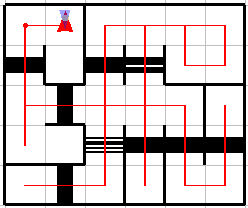
\includegraphics[width=\textwidth]{verkenMap1E}
                \caption{map 1}
        \end{subfigure}%
        \begin{subfigure}[h]{0.36\textwidth}
                \centering
                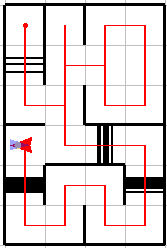
\includegraphics[width=\textwidth]{verkenMap2E}
                \caption{map 2}
        \end{subfigure}
 \caption{Het verkennen van een doolhof met implementatie van aanpassing E. Deze aanpassing maakt dat in map 1 niet alle tegels bezocht hoeven te worden. In map 2 doet deze situatie zich niet voor. Dit is te wijten aan de opbouw van het doolhof.}
\label{fig:resultVerkenE}
\end{figure}

% == het kortste pad == %
\subsection{Het vinden van het kortste pad} % ?
\label{ssec:AlgoKortsteP}

Het kortste pad algoritme maakt gebruik van een graaf die opgesteld wordt tijdens het verkennen van het doolhof. Het algoritme is A* waarbij de Manhattan heuristiek en een kost wordt gebruikt.
De heuristiek is de verwachte afstand tot de "finishTile" en is een onderschatting, er wordt dus geen rekening gehouden met muren. De "finishTile" krijgt de heuristiekwaarde 0, de buren hiervan (horizontaal en verticaal, niet diagonaal) de waarde 1 , enzoverder tot alle tegels een heuristische waarde gekregen hebben.
De kost van een tegel is het werkelijke aantal tegels nodig om van de "startTile" tot de "finishTile" te komen.

In de beginsituatie zijn alle tegels ongemarkeerd en de kost van de "startTile" wordt op nul gezet. Daarna wordt de kost opbouwend aan elke tegel meegegeven. Hierbij worden de muren in rekening gebracht.

Speciaal voor dit algoritme zijn dus 3 extra velden aan de klasse Tile toegevoegd, nl. een booleanveld isMarked dat bijhoudt of dit vakje al “onderzocht” is, een veld dat de heuristiekwaarde bijhoudt en een veld dat de kost van de tile bijhoudt.


% == SOFTWARE == %
\section{Software} % 3 ?
\label{sec:softw}
De software bestaat uit twee delen: een project dat op de NXT van de robot loopt en een project dat op de computer loopt. Alles wordt aangestuurd via de Graphical User Interface (GUI). Deze toepassing laat toe de robot te besturen (via bluetooth) en de reacties van de robot te simuleren met de simulator. Een Communication-pakket stuurt de commando's van de GUI door naar de juiste unit.
De simulator kan gebruikt worden om de software op te testen zonder telkens op de robot te moeten wachten.

% == software design == %
\subsection{Software ontwerp} % 3 ?
\label{ssec:Sdesign}
Zoals reeds vermeld bestaat de software uit twee projecten: \'e\'en draait op een computer en \'e\'en draait op de NXT-Brick. Figuur \ref{fig:klasDia} toont het klassendiagram.\\
Beide projecten hebben een identiek package \textit{commands} met \'e\'en klasse \textit{Command}. Hierin staan de final static integers die met de mogelijke bluetoothsignalen overeenkomen. Een verdere beschrijving van de software op de NXT-brick wordt in de sectie robot gegeven.\\


Het computerproject heeft nog zes andere packages: \textit{communication}, \textit{gui}, \textit{simulator}, \textit{mazeAlgorithm}, \textit{audio} en \textit{mapping}. 
De klasse \textit{SilverSurferGUI} uit de package \textit{gui} implementeert de GUI. De GUI communiceert met de simulator of de robot via de klassen in het package \textit{communication} door een object van de superklasse \textit{UnitCommunicator} bij te houden. Aan deze \textit{UnitCommunicator} is een object van de subklassen \textit{RobotCommunicator} of \textit{SimulatorCommunicator}  toegekend. Zo worden de commands dynamisch naar de juiste unit gestuurd: de \textit{RobotCommunicator} communiceert met het NXT-Project, de \textit{SimulatorCommunicator} met de simulator klassen.\\
Andere klassen van de package \textit{gui} zijn: \textit{MouseClickThread} , \textit{PolygonDrawThread}, \textit{RunForwardThread} en \textit{TurnAngleThread}. De vier Threads zorgen ervoor dat het tekenen van de baan van de robot de rest van het programma niet stillegt. \\

Het package \textit{simulator} implementeert de functionaliteit van de simulator. \\
Het \textit{mapping-package} heeft klassen zoals \textit{Tile, Edge, Obstruction, Barcode, ...} die elementen uit de wereld van een robot voorstellen. Een tile stemt overeen met \'e\'en tegel van het doolhof en heeft vier edges: \'e\'en voor elke zijde. Die edges houden de twee aanliggende tegels bij en eventueel een Obstruction, bijvoorbeeld een muur. De klasse \textit{MapGraph} brengt al deze elementen samen. Het houdt een begin-tegel bij en en huidige-tegel. Het biedt functionaliteiten aan om van de huidige tegel naar de tegel Noord, Oost, Zuid of West ervan te reizen en de map dynamisch uit te breiden. Zo wordt impliciet een hele graaf bijgehouden die dynamisch kan aangevuld worden. De klasse \textit{MapReader} kan uit een bepaalde textfile een MapGraph opstellen die overeenkomt met het doolhof dat in het bestand gedefinieerd wordt.


%figuur klassendiagram PC
\begin{figure}[tbp]
\begin{center}
    \includegraphics[width=0.8\textwidth]{Klassendiagram}
    \caption{Klassendiagram van het project}
    \label{fig:klasDia}
\end{center}
\end{figure}


% == commando's == %
\subsection{Het doorgeven van commando's} % 3 ok!
\label{ssec:commands}
De GUI zet een actie van de gebruiker om in een commando. Dit commando wordt gerepresenteerd door een integer dat naar de \textit{UnitCommunicator} wordt gestuurd. Twee van de commando's hebben echter extra informatie nodig: \textit{automatic move x cm forward} en \textit{rotate x degrees}. Deze informatie wordt toegevoegd aan de integer door de integer uit te breiden met extra cijfers (dit wordt in de volgende sectie in detail beschreven).\\
De \textit{UnitCommunicator} stuurt de bekomen integer door naar ofwel de \textit{RobotCommunicator} ofwel de \textit{SimulatorCommunicator}. Deze zetten de integer weer om in de juiste actie van respectievelijk de robot en de simulator. De wijze waarop dit gebeurt, verschilt licht voor beide gevallen. Zo stuurt de \textit{RobotCommunicator} zijn commando's via Bluetooth door naar de NXT-brick, terwijl de \textit{SimulatorCommunicator} zo'n verbinding niet nodig heeft.\\

\subsubsection{De bewerking op de integers} % 3 ok!
\label{sssec:integer}
Integers stellen de commando's voor. In twee gevallen is echter meer informatie nodig: om de robot een bepaalde afstand te laten afleggen en om de robot een bepaald aantal graden te laten draaien. Deze afstand en dit aantal graden moet mee doorgegeven worden met de integer. De eenheden waarin de afstand en de hoek worden doorgestuurd zijn respectievelijk cm en graden.

De doorgegeven integer wordt als volgt opgebouwd:

\begin{itemize}
\item de waarde van de afstand (hoek) wordt vermenigvuldigd met 1000.
\item de integer die het commando representeert, wordt hierbij opgeteld.
\end{itemize}

Om de bekomen resultaten terug op te splitsen in de twee oorspronkelijke gegevens worden volgende stappen gevolgd:

\begin{itemize}
\item een modulo-operatie van tien geeft het laatste cijfer terug. Dit stelt het soort commando voor.
\item dit getal wordt van de integer terug afgetrokken.
\item de oorspronkelijke afstand (hoek) wordt bekomen door de integer door 1000 te delen.
\end{itemize}

Deze werkwijze brengt een beperking met zich mee: de waarde van de afstand (hoek) kan slechts tot 2 cijfer(s) na de komma doorgegeven worden. De robot kan niet nauwkeuriger dan 0,1 cm aangestuurd worden. Hierdoor is het niet nodig de afstand nauwkeuriger door te geven. De nauwkeurigheid van de hoek is gevoeliger. De veelhoek stapelt immers veel afrondingsfouten op naarmate de lengte van de zijde en/of het aantal hoeken stijgt. Doordat de begin- en eindpunten niet samen vallen is te zien dat de som van de berekende hoeken samen geen 360 graden vormt. 

% == gui == %
\subsection{GUI} % 3 ?
\label{ssec:GUI}
De GUI bestaat uit twee vensters, enkele knoppen, een menubar en enkele instelmogelijkheden: zie figuur \ref{fig:gui}. Deze knoppen besturen ofwel de robot en de simulator ofwel enkel de simulator, naargelang de bluetooth verbinding aan staat. De knoppen voeren bepaalde functies uit, zoals "turn left/right", "look around" en "Align on the white line/ walls".\\

Voor visualisatie van de sensoren zijn er grafieken die de waarden weergeven. De robot zelf op de simulator heeft een blauwe straal die de waarde van de ultrasone sensor aangeeft. 

%figuur gui
\begin{figure}[tbp]
\begin{center}
    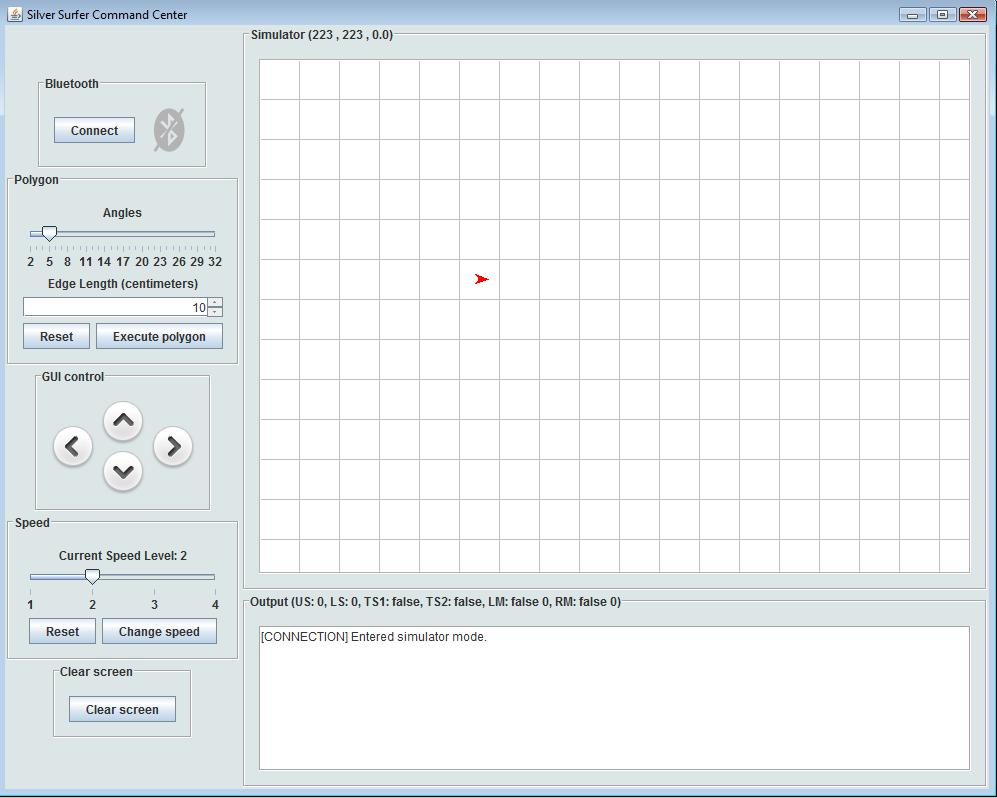
\includegraphics[width=0.8\textwidth]{GUI}
    \caption{Grafische User Interface}
	\label{fig:gui}
\end{center}
\end{figure}

% == bluetooth == %
\subsection{Bluetooth} % 3 ok!
\label{ssec:bluetooth}
De communicatie tussen robot en computer gebeurt volledig via bluetooth. De GUI voorziet een knop om deze verbinding te maken en geeft de status van de verbinding weer. De GUI stuurt commando's door naar de robot via de klassen \textit{UnitCommunicator} en \textit{RobotCommunicator}.

De leJOS-API\^{2} voorziet de \textit{NXTConnector} klasse. De methode \textit{connectTo((String, String, int, int)} zet de bluetoothverbinding tussen computer en brick op. De belangrijkste argumenten hiervoor zijn de naam van de NXT-Brick en zijn DeviceUrl  - in het geval van de gebruikte NXT: 'Silver' en '00:16:53:0A:04:5A'.

De bluetooth laat toe enkele 'datastreams' tussen robot en computer op te zetten. Deze 'datastreams' sturen informatie in verschillende kanalen door. Zo kunnen zowel robot als computer de verschillende 'soorten informatie' van elkaar onderscheiden.

% == robot == %
\subsection{Robot} % 3 ?
\label{ssec:robot}
Het project op de NXT-brick bestaat uit een klasse \textit{CommandUnit}, een klasse \textit{Command} en enkele threadklassen. Deze laatsten maken het mogelijk meerdere dingen tegelijk te doen (bijvoorbeeld: sensorwaarden inlezen terwijl de robot rijdt). Bij het opstarten, initialiseert de robot zijn sensoren. Wanneer de computer verbinding maakt, initialiseert de robot ook zijn 'datastreams' en start hij een \textit{SensorThread} op.

De computer stuurt commando's in de vorm van integers. De robot vertaalt deze met behulp van de klasse \textit{Command} en voert de juiste actie uit. Sommige methodes retourneren een waarde aan de computer. Dit gebeurt door de waarde op een 'datastream' te zetten, voorafgegaan door een tag (bijvoorbeeld: [US] voor ultrasonic sensor data).\\

Enkele belangrijke methodes van \textit{CommandUnit}:
\begin{itemize}
\item \textit{updateCoordinates:} de robot houdt zijn positie bij. bij elke beweging zullen de co\"ordinaten worden ge\"updated.
\item \textit{updateStatus:} stuur alle statusgegevens (lichtsensor, co\"ordinaten, ...) naar de computer.
\item \textit{main:} wacht tot de computer een commando geeft en voer dit uit.
\item \textit{moveForward:} beweegt voorwaarts, maar stopt bij een barcode.
\end{itemize}

De \textit{SensorThread} stuurt elke 50 milliseconden sensorinformatie door naar de computer. Zo blijft de data up to date zonder dat de 'datastream' te veel informatie moet slikken.

% == simulator == %
\subsection{Simulator} % 3 ?
\label{ssec:simulator}
De simulator bootst de werking van de robot virtueel na. Hij kan dezelfde commando's uitvoeren als de werkelijke robot. De GUI stuurt de simulator aan via de klassen \textit{UnitCommunicator} en \textit{SimulatorCommunicator}. Deze ontvangen de uit te voeren commando's, analyseren ze en sturen ze door naar de simulator.
\\
De simulator zelf bestaat uit zeven klassen:

% overzicht klassen simulator
\begin{itemize}
\item \textit{Wall:} tekent de muren van het doolhof.
\item \textit{State:} wordt gebruikt om te zeggen of iets horizontaal of verticaal moet staan.
\item \textit{SimulationSensorData: }
\item \textit{SimulationPilot:} houdt de positie en de richting van de 'robot' bij.
\item \textit{SimulationPanel:} tekent de baan van de 'robot' in het tekenpaneel.
\item \textit{Triangle:} berekent de hoekpunten van de driehoek die de 'robot' voorstelt.
\item \textit{ExtMath:} doet enkele berekeningen.
\item \textit{Bag:\cite{Bag.java} } een geheugen opslagplaats waar dubbels in worden opgeslagen.
\end{itemize}

Het opzetten van het tekenpaneel gebeurt in de klasse \textit{SilverSurferGUI}. De roosters op het achtergrond van het tekenpaneel hebben dezelfde afmetingen als de secties van de panelen. Zo kan een muur enkel op een lijn van het grid staan.
Wanneer de 'robot' een pad aflegt, tekent de simulator dit in het tekenpaneel als een rode lijn (herschaald: \'e\'en cm = \'e\'en pixel). De lijn  bestaat uit verschillende cirkels die elkaar gedeeltelijk overlappen. Het \textit{SimulationPanel} houdt alle bezochte co\"ordinaten bij. De klasse bevat een methode die deze cirkels \'e\'en na \'e\'en tekent. Dit zorgt ervoor dat de lijn continu bijgewerkt wordt. De huidige positie en de huidige orientatie van de 'robot' wordt bovenaan het simulatorpaneel in de GUI weergegeven.

% == BESLUIT == %
\section{Besluit} % 3 ?
\label{sec:besl}
De uiteindelijke fysieke bouw van de robot bestaat uit de NXT, de wielen met aandrijvingen, een ultrasone sensor, een lichtsensor en twee druksensoren.
De calibratie van de robot zorgt ervoor dat hij precies aangestuurd kan worden en dat de sensoren waarden teruggeven die overeenkomen met de werkelijkheid.
De GUI gebruikt een eenvoudige interface en bevat knoppen waarmee de robot handmatig bestuurd kan worden. Door het ingeven van parameters in de GUI kan de robot een willekeurige veelhoek rijden. De uitleeswaarden van de sensoren vertellen de gebruiker wat de robot 'ziet'. Op deze manier krijgt de gebruiker een idee over de doolhof waar de robot in rijdt. Bovendien kan de robot zich loodrecht ori\"enteren op een witte lijn. De simulator is ook verbonden aan de GUI. Deze voert dezelfde opdracht uit als de robot. Het is mogelijk een virtueel doolhof te laten en de simulator hier in te laten 'rijden'. De simulator is handig om testen op uit te voeren, zonder steeds op de robot te moeten wachten.


\newpage
\makeappendix

% == DEMO 1 == %
\section{Demo 1} % 3 ?
\label{Asec:demo1}
De robot wordt voor demo 1 nog niet voorzien van sensoren. De focus ligt vooral op de nauw-
keurigheid van de besturing en op het implementeren van alle softwarecomponenten. Deze software
bestaat uit twee projecten: een op de computer en een op de robot. De computersoftware bestaat
uit een Grafical User Interface (GUI), enkele Communication klassen die informatie doorsturen en
enkele klassen die de werking van de robot simuleren (simulator).

% == resulaten == %
\subsection{Resultaten} % 3 ?
\label{Assec:result1}
Bij het rijden van de veelhoek had de robot een kleine afwijking. De afwijking werd groter bij grotere veelhoeken en meerdere hoeken om wille van de geaggregeerde fout.

% == conclusies == %
\subsection{Conclusies} % 3 ?
\label{Assec:conc1}
Calibratie moet meer getest worden. De GUI kan gebruiksvriendelijker, ook moet het scherm van de simulator herschaald worden, zodat de lijn van simulator nog wordt weergegeven als de simulator van de robot uit het scherm gaat.

% == aanpassingen == %
\subsection{Oplijsting aanpassingen verslag} % 3 ?
\label{Assec:aanp1}
Volgende secties werden aangepast ten opzichte van de eerste demonstratie:

% overzicht aangepaste secties
\begin{itemize}
\item \textit{\ref{ssec:fysbouw} Fysieke bouw:} de sensoren werden toegevoegd.
\item \textit{\ref{ssec:calibM} Calibratie van de motoren:} opnieuw gedaan.
\item \textit{\ref{ssec:calibLS} Calibratie van de lichtsensor:} nieuwe sectie.
\item \textit{\ref{ssec:calibUS} Calibratie van de ultrasone sensor:} nieuwe sectie.
\item \textit{\ref{ssec:algoVeelH} Het rijden van een veelhoek:} nieuwe sectie.
\item \textit{\ref{ssec:algoWitteL} Het rechtzetten op een witte lijn:} nieuwe sectie.
\item \textit{\ref{ssec:Sdesign} Software ontwerp:} enkele nieuwe klassen en mapping-package.
\item \textit{\ref{ssec:GUI} GUI:} enkele nieuwe functionaliteiten.
\item \textit{\ref{ssec:simulator} Simulator:} grid en triangle, virtuele doolhof.
\end{itemize}


% == DEMO 2 == %
\section{Demo 2} % 3 ?
\label{Asec:demo2}
De sensoren worden voor demo 2 wel ge\"installeerd. Na calibratie kunnen ze informatie doorzenden naar de robot. Threads zorgen ervoor dat de robot tegelijkertijd sensorwaarden kan lezen doorsturen.\\

De meetwaarden worden in de GUI weergegeven zodat een gebruiker de robot kan besturen zonder deze te zien. Bovendien is de simulator gekoppeld aan de robot. Wat de robot doet, doet de simulator ook en wordt getekend in de GUI. De simulator kan ook onafhankelijk van de robot opereren. Het is mogelijk een virtuele doolhof te laden en te simuleren dat de 'robot' zich hierdoor beweegt. Zowel robot als simulator kunnen zich rechtzetten op een (virtuele) witte lijn. Het is bovendien mogelijk de robot zich in het midden van de tegel te laten zetten.


% == resulaten D2== %
\subsection{Resultaten} % 3 ?
\label{Assec:result2}
Het verslag voor de tweede demonstratie bevatte enkele paragrafen die tegen het einde nog snel geschreven waren. Deze paragrafen waren van mindere kwaliteit. Ook sommige afbeeldingen werden verkeerd ingevoegd.\\

Op de demonstratie reed de robot de eerste tegels zoals het hoorde. Ook het witte lijnalgoritme werd goed uitgevoerd. De sensorwaarden werden weergegeven in de GUI, zodat de bestuurder, die de robot en het doolhof niet zag, zich een beeld kon vormen van het doolhof. Op een gegeven moment gaf de bestuurder de robot opdracht zich midden op een tegel te zetten. Dit algoritme maakt gebruik van de muren rond de tegel. De robot bevond zich op dat ogenblik echter op een tegel die door geen enkele muur omsloten werd. De bestuurder had dit niet eerst nagekeken. Dit had als gevolg dat de robot helemaal scheef stond, zonder dat de bestuurder dit wist.\\

De sensorwaarden werden niet gesimuleerd in de simulator. De simulator maakte in zijn algoritmes rechtstreeks gebruik van de virtuele doolhof. Robot en simulator maakten met andere woorden gebruik van andere algoritmes, wat niet het doel is van een simulator.\\

De simulator kon wel door een virtuele doolhof manoeuvreren. Meestal 'botste' hij tegen de muren, maar soms reed hij toch door een muur.


% == conclusies D2== %
\subsection{Conclusies} % 3 ?
\label{Assec:conc2}
Aan het verslag zou vroeger begonnen moeten worden zodat domme fouten vermeden kunnen worden.

De allign-algoritmes (op een witte lijn en in het midden van een tegel) werken enkel in specifieke situaties. De algoritmes dienen enkel in deze omstandigheden uitgevoerd te worden.

De simulator dient de sensorwaarden te simuleren en zou dezelfde algoritmes moeten gebruiken als de robot. Op deze manier kunnen de algoritmes getest worden zonder steeds op de robot te wachten.


% == aanpassingen D2== %
\subsection{Oplijsting aanpassingen verslag} % 3 ?
\label{Assec:aanp2}
Volgende secties werden aangepast ten opzichte van de tweede demonstratie:

% overzicht aangepaste secties D2
\begin{itemize}

\item \textit{\ref{ssec:abstr} Abstract:} aangepast.
\item \textit{\ref{ssec:calibLS} Calibratie van de lichtsensor:} meetresultaten toegevoegd.
\item \textit{\ref{ssec:calibUS} Calibratie van de ultrasone sensor:} meetresultaten toegevoegd en aangepast.
\item \textit{ Het rijden van een veelhoek:} er uitgehaald.
\item \textit{\ref{ssec:algoWitteL} Het rechtzetten op een witte lijn:} aangepast.
\item \textit{\ref{ssec:algoOnderzDoolhof} Algoritme onderzoeken doolhof:} nieuwe sectie.
\item \textit{\ref{ssec:AlgoKortsteP} Algoritme Kortste pad:} nieuwe sectie.
\item \textit{\ref{ssec:Sdesign} Software ontwerp:} enkele nieuwe klassen en packages.
\item \textit{\ref{ssec:GUI} GUI:} aangepast.
\item \textit{\ref{ssec:simulator} Simulator:} toevoegingen.
\end{itemize}

% == DEMO 3 == %
%\section{Demo 3} % 3 ?
%\label{Asec:demo3}

% == resulaten D3 == %
%\subsection{Resultaten} % 3 ?
%\label{Assec:result3}

% == conclusies D3== %
%\subsection{Conclusies} % 3 ?
%\label{Assec:conc3}

% == aanpassingen D3== %
%\subsection{Oplijsting aanpassingen verslag} % 3 ?
%\label{Assec:aanp3}
%Volgende secties werden aangepast ten opzichte van de eerste demonstratie:

% overzicht aangepaste secties
%\begin{itemize}
%\end{itemize}



\begin{thebibliography}{9}

\bibitem{mindstorms}
\textit{Lego Mindstorms}:  Een uitbreiding op de LEGO bouwstenen waarmee kleine, aanpasbare en programmeerbare robots gebouwd kunnen worden. Een centrale besturingsmodule ('the brick') kan geprogrammeerd worden met verschillende programmeertalen. In eerdere versies werd een RCX gebruikt voor de brick, nu wordt met NXT gewerkt. De brick kan enkele motoren aandrijven. Bovendien kunnen er verschillende sensoren, o.a. een ultrasone sensor en een lichtsensor, aangesloten worden.  \mbox{[www.lego.com]} \mbox{[http://en.wikipedia.org/wiki/Lego\textendash Mindstorms]}

\bibitem{leJOS}
\textit{leJOS}:  Een kleine Java Virtuele Machine die toelaat de NXT-brick te programmeren. leJOS voorziet verschillende klassen die o.a. de motoren aansturen en een bluetoothverbinding opzetten.  \mbox{[http://lejos.sourceforge.net/]}

\bibitem{Bag.java}
\textit{Bag.java}: Voor meer documentatie, zie naar http://algs4.cs.princeton.edu/13stacks. \\
Section 1.3 of "Algorithms, 4th Edition" door Robert Sedgewick en Kevin Wayne.

\end{thebibliography}

\end{document}

